\chapter{Aan de slag}\addtocontents{toc}{\protect\setcounter{tocdepth}{2}}
\hypersetup{bookmarksdepth=5}

\section{Toetsenbord}
\label{cha:getting-started}
\index{Toetsenbord}

Nu alles is aangesloten, is het tijd om vertrouwd te raken met het toetsenbord van de MEGA65.

Wellicht valt u op dat het toetsenbord enigszins afwijkt van de toetsenborden van andere hedendaagse computers. De meeste toetsen staan op vertrouwde posities, maar er zijn enkele gespecialiseerde toetsen en sommige toetsen hebben speciale grafische symbolen op de voorkant.

In sommige beeldschermmodi zijn de grafische symbolen te typen, net als letters, cijfers en leestekens. De volledige verzameling tekens staat bekend als de {\em PETSCII-tekenset}.\index{PETSCII}

\subsection{Speciale toetsen}

\subsubsection{RETURN}
\index{Toetsenbord!RETURN}
Wanneer u op \specialkey{RETURN} drukt, slaat de computer de informatie die u hebt getypt op in het geheugen. De computer voert vervolgens een opdracht uit, bewaart enkele gegevens of toont een foutmelding indien u een vergissing hebt gemaakt.

\subsubsection{SHIFT}
\index{Toetsenbord!Shifttoetsen}
De twee \specialkey{SHIFT}-toetsen bevinden zich links en rechts. Zij werken vrijwel hetzelfde als de Shift-toets van een gewoon toetsenbord en vervullen daarnaast nog enkele speciale functies.

In de modus met hoofdletters levert het ingedrukt houden van \specialkey{SHIFT} en het indrukken van een toets met twee grafische symbolen op de voorkant het rechter symbool van die toets op. Zo toont \specialkey{SHIFT} samen met \megakey{J} het teken \graphicsymbol{J}.

In de modus met kleine letters geeft het indrukken van \specialkey{SHIFT} en een lettertoets de hoofdletter van die toets weer.

Om de Griekse letter $\pi$ (pi) te typen, houdt u \specialkey{SHIFT} ingedrukt en drukt u op \megakeywhite{$\uparrow$}.

Het ingedrukt houden van \specialkey{SHIFT} en het indrukken van een functietoets roept de functie op die op de voorkant van die toets staat vermeld. Zo activeert \specialkey{SHIFT} samen met \megakey{F1} de functie \megakey{F2}.


\subsubsection{SHIFT LOCK}
\index{Toetsenbord!SHIFT LOCK}
Naast \specialkey{SHIFT} is er de \specialkey{SHIFT\\LOCK}-toets. Druk op deze toets om de Shift-functie vast te zetten. Wanneer \specialkey{SHIFT\\LOCK} verlicht is, toont elke toets die u indrukt het bijbehorende teken op het scherm, alsof u \specialkey{SHIFT} ingedrukt houdt. Dit geldt ook voor speciale grafische tekens.

\subsubsection{CTRL}
\index{Toetsenbord!CTRL}
\specialkey{CTRL} is de Control-toets. Door \specialkey{CTRL} ingedrukt te houden en een andere toets in te drukken, kunt u Controlcodes uitvoeren. Zo kunt u met \specialkey{CTRL} ingedrukt en één van de cijfertoetsen (van \megakey{1} tot \megakey{8}) de tekstkleur wijzigen. De kleur die op de bovenste rij van de voorkant van de cijfertoets is afgedrukt, wordt gebruikt. Het ingedrukt houden van \specialkey{CTRL} en het indrukken van \megakey{9} of \megakey{0} schakelt de modus voor omgekeerde tekst in en uit.

Enkele voorbeelden hiervan vindt u op bladzijde \pageref{sec:screen-editor} en alle Controlcodes staan vermeld op bladzijde \pageref{appendix:controlcodes}.

Wanneer een programma met {\bf LIST} op het scherm wordt weergegeven, vertraagt het ingedrukt houden van \specialkey{CTRL} de weergave van elke regel. Meer over het commando {\bf LIST} leest u op bladzijde \pageref{BASIC 65 Commands!LIST}.\index{BASIC 65-commando's!LIST}

Het ingedrukt houden van \specialkey{CTRL} en het indrukken van \megakey{*} opent de Matrix Mode Debugger (raadpleeg {\bf Het grote Mega65-boek} voor meer details).

\subsubsection{RUN/STOP}
\index{Toetsenbord!RUN STOP}
Normaal gesproken stopt het indrukken van \specialkey{RUN\\STOP} de uitvoering van een programma. Wanneer u \specialkey{SHIFT} ingedrukt houdt en op \specialkey{RUN\\STOP} drukt, voert u met {\bf RUN} het eerste programma van de schijf uit.\index{BASIC 65-commando's!RUN}

Sommige programma's onderscheppen de \specialkey{RUN\\STOP}-toets en kunnen op deze wijze niet worden gestopt.

U kunt uw MEGA65 naar de {\bf Machinetaalmonitor}\index{Machinetaalmonitor} opstarten door \specialkey{RUN\\STOP} ingedrukt te houden en de resetknop aan de linkerkant van de computer in te drukken (of door de toets ingedrukt te houden terwijl u de computer inschakelt).

\subsubsection{RESTORE}
\index{Toetsenbord!RESTORE}
Het computerscherm kan naar een schone toestand worden teruggebracht zonder het geheugen te wissen door \specialkey{RUN\\STOP} ingedrukt te houden en \widekey{RESTORE} in te drukken. Deze combinatie herstelt tevens de vectoren van het besturingssysteem en initialiseert de schermeditor opnieuw, hetgeen dit tot een handige combinatie maakt indien de computer een beetje in de war is geraakt.

Sommige programma's onderscheppen de toetsencombinatie \specialkey{RUN\\STOP} + \widekey{RESTORE} en kunnen op deze wijze niet worden gereset.

U kunt de {\bf Freezer} ook oproepen door \widekey{RESTORE} één seconde ingedrukt te houden en de toets vervolgens los te laten. U kunt meer over de Freezer lezen op bladzijde \pageref{sec:freezer}.\index{Freezer-menu}

\subsubsection{De cursor-toetsen}
\index{Toetsenbord!Cursortoetsen}
\nopagebreak
De cursor-toetsen staan rechtsonder op het toetsenbord. Met deze vier richtingtoetsen kunt u de cursor naar elke gewenste positie verplaatsen voor het bewerken van tekst op het scherm.

De cursor beweegt in de richting die op de toetsen is aangegeven: \megakey{$\leftarrow$} \megakey{$\uparrow$} \megakey{$\rightarrow$} \megakey{$\downarrow$}.

U hoeft een cursor-toets niet telkens opnieuw in te drukken. Indien u de cursor over een grote afstand moet verplaatsen, kunt u de toets ingedrukt houden. Wanneer u klaar bent, laat u de toets gewoon los.

\subsubsection{De pijltjestoetsen}
\index{Toetsenbord!Pijltjestoetsen}
Deze toetsen verschillen van de cursor-toetsen. Het zijn \megakeywhite{$\leftarrow$} (naast \megakey{1}) en \megakeywhite{$\uparrow$} (naast \widekey{RESTORE}). Beide pijltjestoetsen worden gebruikt in diverse BASIC-functies en escape-sequenties.

Zo kan \megakeywhite{$\leftarrow$} als snelkoppeling voor {\bf SAVE}\index{BASIC 65-commando's!SAVE} dienen en wordt \megakeywhite{$\uparrow$} gebruikt om een getal tot een macht te verheffen (hetgeen gelijkstaat aan het getal een opgegeven aantal malen met zichzelf te vermenigvuldigen).

U kunt meer lezen over de beschikbare escape-sequenties op bladzijde \pageref{escape-sequences}.

Deze twee PETSCII-specifieke toetsen worden in de MEGA65-literatuur altijd met een witte achtergrond weergegeven.

Het is ook mogelijk de cursor met \specialkey{SHIFT} en \megakey{$\downarrow$} omhoog en met \specialkey{SHIFT} en \megakey{$\rightarrow$} naar links te verplaatsen. Dit is een erfenis van de Commodore 64, welke slechts twee cursor-toetsen had.

\subsubsection{INSerT/DELete}
\index{Toetsenbord!INST DEL}
De toets \specialkey{INST\\DEL}, de meest rechtse toets van de bovenste rij, is de INSERT/DELETE-toets. Wanneer u \specialkey{INST\\DEL} indrukt, wordt het teken links daarvan verwijderd en worden alle tekens rechts daarvan één positie naar links verschoven.

Om een teken in te voegen, houdt u \specialkey{SHIFT} ingedrukt en drukt u op \specialkey{INST\\DEL}. Het teken onder de cursor en de tekens rechts van de cursor worden naar rechts verschoven. Op de nieuw vrijgekomen plaats kunt u vervolgens een letter, een cijfer of elk ander teken typen.


\subsubsection{CLeaR/HOME}
\index{Toetsenbord!CLR HOME}
De toets \specialkey{CLR\\HOME} is de CLEAR/HOME-toets. Het indrukken van \specialkey{CLR\\HOME} verplaatst de cursor naar de linkerbovenhoek van het scherm.

Door \specialkey{SHIFT} ingedrukt te houden en op \specialkey{CLR\\HOME} te drukken, wist u het volledige scherm {\it en} plaatst u de cursor in de linkerbovenhoek van het scherm.

Indien u per ongeluk \specialkey{CLR\\HOME} indrukt, kunt u de cursor naar zijn vorige positie terugbrengen door \specialkey{ESC} en vervolgens \specialkey{CLR\\HOME} in te drukken.

\subsubsection{De MEGA-toets}
\index{Toetsenbord!MEGA-toets}
De \megasymbolkey of de MEGA-toets biedt een aantal verschillende functies en kan worden gebruikt om speciale hulpprogramma's op te starten.

Door \specialkey{SHIFT} ingedrukt te houden en \megasymbolkey in te drukken, schakelt u tussen de kleine- en de hoofdlettermodus.

Door \megasymbolkey ingedrukt te houden en een willekeurige toets met twee grafische symbolen op de voorkant in te drukken, geeft de computer het meest linkse grafische symbool op het scherm weer. Zo geven \megasymbolkey en \megakey{D} het symbool \graphicsymbol{d} weer.

Door \megasymbolkey ingedrukt te houden en een cijfertoets in te drukken, schakelt u over naar een secundaire kleur, d.w.z. de kleur die op de onderste rij aan de voorkant van de cijfertoets is afgedrukt.

Door \megasymbolkey ingedrukt te houden en \specialkey{TAB} in te drukken, opent u de Matrix Mode Debugger (zie voor meer details {\bf Het grote Mega65-boek}).

Indien u de MEGA65 inschakelt, of de resetknop aan de linkerkant indrukt terwijl u \megasymbolkey ingedrukt houdt, schakelt de MEGA65 over naar de GO64-modus.\index{Commodore 64!GO64-modus}

\subsubsection{NO SCROLL}
\index{Toetsenbord!NO SCROLL}
Indien een programma met {\bf LIST} naar het scherm wordt afgedrukt, onderbreekt u de schermuitvoer door \specialkey{NO\\SCROLL} in te drukken. Druk een willekeurige toets in om de pauze op te heffen.

Deze functie is niet beschikbaar in de GO64-modus.\index{Commodore 64!GO64-modus}

\subsubsection{De functietoetsen}
\index{Toetsenbord!Functietoetsen}
Er zijn zeven functietoetsen beschikbaar die door softwaretoepassingen gebruikt kunnen worden. \megakey{F1} \megakey{F3} \megakey{F5} \megakey{F7} \megakey{F9} \megakey{F11} en \megakey{F13} kunnen worden gebruikt om speciale functies uit te voeren.

Houd \specialkey{SHIFT} ingedrukt om \megakey{F2} tot en met \megakey{F14} te gebruiken, zoals op de voorkant van elke functietoets is aangegeven.
\index{Toetsenbord!Shifttoetsen}
In de GO64-modus zijn alleen de functietoetsen \megakey{F1} tot en met \megakey{F8} beschikbaar.\index{Commodore 64!GO64-modus}

\subsubsection{HELP}
\index{Toetsenbord!HELP}
\specialkey{HELP} kan door software worden gebruikt en fungeert tevens als \megakey{F15}.

\subsubsection{ALT}
\index{Toetsenbord!ALT}
Software kan specifieke functies uitvoeren door \specialkey{ALT} ingedrukt te houden en tegelijkertijd andere toetsen in te drukken. Deze functie is niet beschikbaar in de GO64-modus.\index{Commodore 64!GO64-modus}

Door \specialkey{ALT} ingedrukt te houden terwijl u de MEGA65 inschakelt, opent u het hulpprogrammamenu.\index{Hulpprogrammamenu} U kunt een SD-kaart formatteren, het MEGA65-configuratiehulpprogramma\index{Configuratie!Hulpprogramma} openen om de standaard videomodus te kiezen en andere instellingen te wijzigen, of uw toetsenbord testen.

\subsubsection{CAPS LOCK}
\index{Toetsenbord!CAPS LOCK}
\specialkey{CAPS\\LOCK} werkt op dezelfde wijze als \specialkey{SHIFT\\LOCK} in de C65- en MEGA65-modus, maar heeft alleen invloed op de lettertoetsen.

Indien de MEGA65 is ingesteld om op een lagere processorsnelheid te draaien, zoals in de GO64-modus,\index{Commodore 64!GO64-modus} kunt u \specialkey{CAPS\\LOCK} ingedrukt houden om de processor tijdelijk op volledige snelheid te laten draaien. Dit is in de GO64-modus nuttig om bijvoorbeeld het laden vanaf het interne schijfstation of de SD-kaart te versnellen, of om het uitpakproces na het uitvoeren van een programma aanzienlijk te versnellen. De MEGA65-modus draait standaard op maximale snelheid.

\addtocontents{toc}{\protect\setcounter{tocdepth}{5}}


\section{De schermeditor}
\label{sec:screen-editor}

Wanneer u uw MEGA65 inschakelt of reset, verschijnt het volgende scherm:\footnote{Hiervoor moet u het Intro Disk-menu hebben uitgeschakeld. Indien het Intro Disk-menu draait, drukt u op ``/'' (schuine streep) om naar dit scherm terug te keren.}

\begin{center}
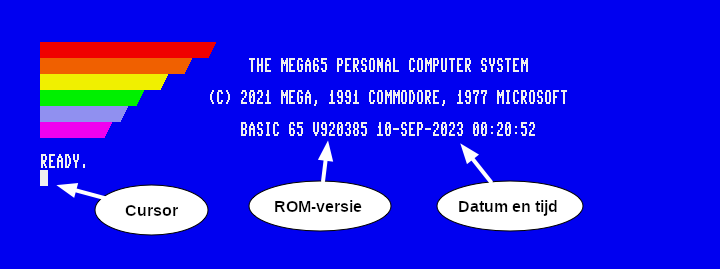
\includegraphics[width=0.9\linewidth]{dutch/images/introduction-screen/layout.png}
\end{center}

De kleurbalken linksboven in het scherm kunt u gebruiken als richtlijn om de kleuren van uw beeldscherm te kalibreren. Het scherm toont tevens de naam van het systeem, de copyrightmelding en de ROM-versie. De weergegeven datum en tijd zijn afkomstig van de interne RTC (Real-Time Clock) op het moment dat de computer werd ingeschakeld. U kunt de datum en tijd instellen in het configuratiehulpprogramma.

Ten slotte ziet u de \screentext{READY}-prompt en de knipperende cursor.

U kunt beginnen met typen op het toetsenbord en de tekens verschijnen op de cursorpositie. Na elke toetsaanslag schuift de cursor één positie verder.

U kunt ook omgekeerde tekst of kleurbalken maken door \specialkey{CTRL} ingedrukt te houden en \megakey{9} of \megakey{R} in te drukken. Hiermee schakelt u de modus voor omgekeerde tekst in. Indien deze modus is ingeschakeld, kunt u de spatiebalk \megakey{Space} indrukken en ingedrukt houden. Terwijl u dat doet, wordt een witte balk over het scherm getekend.
\index{Toetsenbord!CTRL}
U kunt de huidige kleur wijzigen door \specialkey{CTRL} ingedrukt te houden en een cijfertoets in te drukken (van \megakey{1} tot \megakey{8}). Indien u bijvoorbeeld \specialkey{CTRL} ingedrukt houdt en \megakey{1} indrukt, verandert de kleur in zwart. Wanneer u nu de spatiebalk \megakey{Space} ingedrukt houdt, wordt een zwarte balk getekend. Indien u de kleur blijft wijzigen en de spatiebalk \megakey{Space} indrukt, krijgt u een effect dat vergelijkbaar is met de volgende afbeelding:

\begin{center}
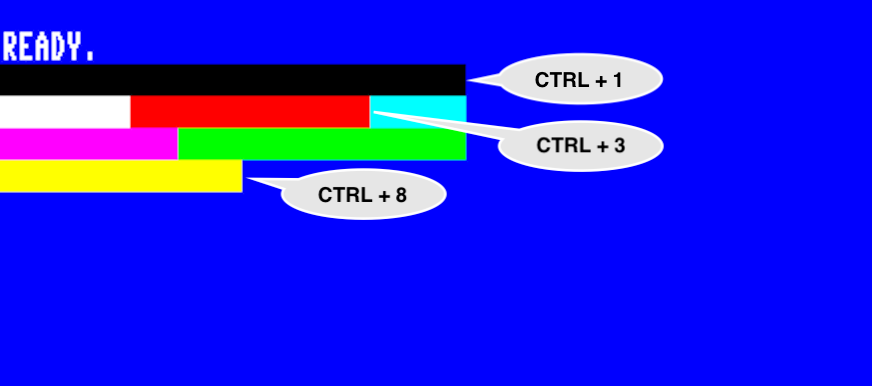
\includegraphics[width=0.7\linewidth]{images/introduction-screen/colour-bars.png}
\end{center}

U kunt de modus voor omgekeerde tekst uitschakelen door \specialkey{CTRL} ingedrukt te houden en \megakey{0} in te drukken.

Nog acht kleuren kunt u selecteren door \megasymbolkey ingedrukt te houden en een toets van \megakey{1} tot \megakey{8} in te drukken.\index{Toetsenbord!MEGA-toets}

De kleur die op de onderste rij aan de voorkant van de cijfertoets is afgedrukt, wordt gebruikt. Indien u bijvoorbeeld \megasymbolkey ingedrukt houdt terwijl u \megakey{4} indrukt, wordt donkergrijs gebruikt. Voor toegang tot nog 16 kleuren van het alternatieve/rainbow-palet verwijzen wij u naar de sneltoets \specialkey{CTRL} + \megakey{A}, die beschreven staat op bladzijde \pageref{appendix:controlcodes}.

\underline{OPMERKING}:
\begin{itemize}
  \item {\bf Zinnebeeldmodus}: Indien u \megakey{"} indrukt om een tekenreeks te beginnen en vervolgens probeert kleuren te wijzigen, tekst om te keren, de cursor te verplaatsen of de toets \specialkey{CLR\\HOME} te gebruiken, verschijnen er in plaats van dat deze acties onmiddellijk plaatsvinden, grappige PETSCII\index{PETSCII}-tekens. Dit komt door een voorziening van BASIC die {\it zinnebeeldmodus} heet en waarmee u dergelijke acties in een tekenreeks kunt coderen, zodat u ze op een later tijdstip kunt uitvoeren (bijvoorbeeld via een {\bf PRINT}-instructie in uw programma's). Om de zinnebeeldmodus te beëindigen typt u eenvoudig een nieuwe \megakey{"} om het einde van uw tekenreeks aan te geven.  \item {\bf Invoegmodus}: Een vergelijkbare voorziening is de {\it invoegmodus}. Het aantal keren dat u \specialkey{SHIFT} + \specialkey{INST\\DEL} indrukt om enkele spaties in te voegen, is gelijk aan het aantal toetsaanslagen dat erop volgt en dat zich volgens dezelfde beginselen als de zinnebeeldmodus gedraagt.  \item U kunt beide modi ook geforceerd beëindigen door \specialkey{ESC} en daarna \megakey{O} in te drukken.
\end{itemize}

\needspace{4cm}
U kunt eenvoudig leuke afbeeldingen maken door deze kleuren en letters te gebruiken. Hieronder ziet u een voorbeeld van wat een vierdejaarsstudent tekende:

\begin{center}
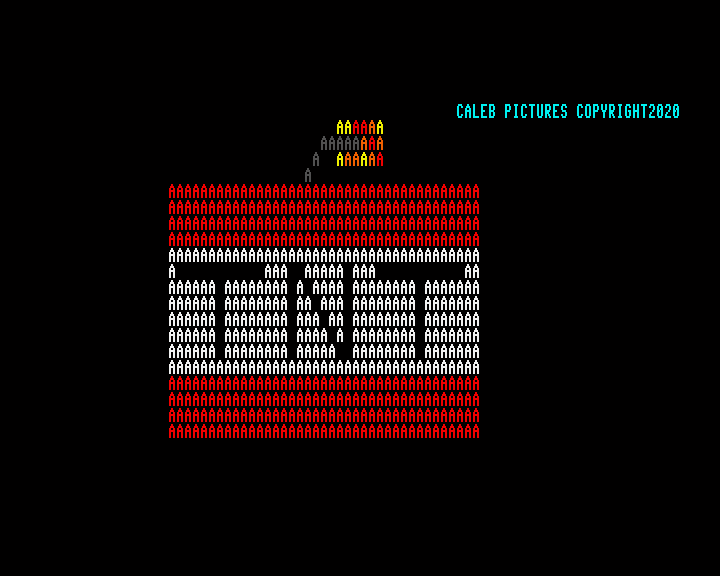
\includegraphics[width=0.7\linewidth]{images/caleb-PETSCII-TNT-final}
\end{center}

Wat gaat u tekenen?

\needspace{2cm}
\textbf{Functies}

Functies die gebruikmaken van \specialkey{CTRL} worden \textbf{Controlcodes} genoemd. Functies die gebruikmaken van \megasymbolkey worden \textbf{Megacodes} genoemd. Er bestaan ook functies die via \specialkey{SHIFT} worden aangeroepen; deze worden \textbf{Shiftcodes} genoemd.

Ten slotte maakt \specialkey{ESC} het gebruik van \textbf{escape-sequenties} mogelijk.

Over al deze functies leest u meer op bladzijde \pageref{appendix:controlcodes}.

\needspace{2cm}
\textbf{Escape-sequenties}

\index{Toetsenbord!Escape-reeksen}
Escape-sequenties worden iets anders uitgevoerd dan een controlcode of een shiftcode. In plaats van de modificatietoets ingedrukt te houden, voert u een escape-sequentie uit door \specialkey{ESC} in te drukken, deze los te laten en vervolgens de gewenste toets in te drukken.

Om bijvoorbeeld te schakelen tussen de 80-kolomsmodus en de 40-kolomsmodus drukt u \specialkey{ESC} in, laat u deze los en drukt u vervolgens op \megakey{X}.

Er zijn nog meer tekstmodi beschikbaar. U kunt knipperende tekst maken door \specialkey{CTRL} ingedrukt te houden en op \megakey{O} te drukken. Alle tekens die u intypt, zullen knipperen. Schakel de knippermodus uit door \specialkey{ESC} en daarna \megakey{O} in te drukken.


\section{Functionaliteit van de editor}

De schermeditor van de MEGA65\index{Schermeditor} biedt verschillende manieren om de cursor snel over het scherm te verplaatsen, zodat u productiever kunt werken.

Druk bijvoorbeeld op \specialkey{CLR\\HOME} om naar de startpositie op het scherm te gaan. Houd \specialkey{CTRL} ingedrukt en druk enkele malen op \megakey{W}. Dit is de functie \textbf{Word Advance}, die uw cursor naar het volgende woord of afdrukbare teken verplaatst.

U kunt naar eigen inzicht tabposities op het scherm instellen. Druk op \specialkey{CLR\\HOME} en vervolgens op \megakey{$\rightarrow$} om de cursor naar de vierde kolom te verplaatsen. Houd \specialkey{CTRL} ingedrukt en druk op \megakey{X} om een tab in te stellen. Verplaats de cursor nog 16 posities naar rechts en druk opnieuw op \specialkey{CTRL} en \megakey{X} om een tweede tab in te stellen.

Druk op \specialkey{CLR\\HOME} om terug te keren naar de startpositie. Houd \specialkey{CTRL} ingedrukt en druk op \megakey{I}. Dit is de functie \textbf{Forward Tab}. Uw cursor springt naar de vierde positie. Druk opnieuw op \specialkey{CTRL} en \megakey{I}. Uw cursor verplaatst zich naar positie 8. Standaard is elke achtste positie reeds als tabpositie ingesteld. De vierde en de twintigste positie zijn derhalve toegevoegd aan de bestaande tabposities. U kunt op \specialkey{CTRL} en \megakey{I} blijven drukken om door te springen naar de zestiende en twintigste positie.

\subsection{Een venster maken}
\index{Toetsenbord!Escape-reeksen}
\index{Vensters!Escape-reeksen}

U kunt een venster instellen op het werkscherm van de MEGA65. Verplaats uw cursor naar het begin van de tekst ``BASIC 65''. Druk op \specialkey{ESC} en daarna op \megakey{T}. Verplaats de cursor 10 regels omlaag en 15 posities naar rechts.

Druk op \specialkey{ESC} en daarna op \megakey{B}. Alles wat u typt, blijft binnen dit venster.

Indien u bijvoorbeeld \screentext{LIST} typt om een programma weer te geven, blijft de listing beperkt tot het venstergedeelte dat u hebt aangegeven:

\begin{center}
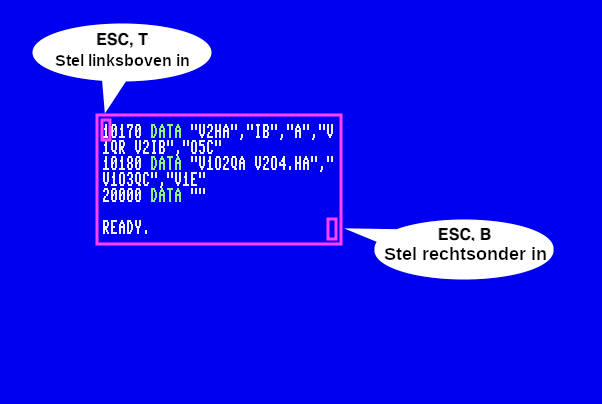
\includegraphics[width=0.7\linewidth]{dutch/images/set-window.png}
\end{center}

Druk tweemaal op \specialkey{CLR\\HOME} om het venster te verlaten en terug te keren naar het volledige scherm.

\subsection{Aanvullende ASCII-tekens}

U hebt misschien opgemerkt dat zich op het toetsenbord van de MEGA65 een aantal ASCII-tekens bevindt die van oudsher geen deel uitmaken van de PETSCII-tekenset\index{PETSCII}. Om deze tekens te gebruiken:

\begin{itemize}
  \item Typ \screentext{FONT A} of \screentext{FONT B}.  \item Druk op \megasymbolkey + \specialkey{SHIFT} om over te schakelen naar kleine letters.
\end{itemize}

U kunt die extra ASCII-tekens nu typen door \megasymbolkey ingedrukt te houden en de toets in te drukken.

\begin{center}
  \begin{tabular}{|l|c|l|}
  \hline
  \textbf{Naam} & \textbf{Teken} & \textbf{Toetscombinatie} \\
  \hline
  Backtick & \texttt{\`} & \megasymbolkey + \megakeywhite{$\leftarrow$} \\
  \hline
  Tilde & \texttt{\~} & \megasymbolkey + \megakey{,} (komma) \\
  \hline
  Verticale streep & \texttt{|} & \megasymbolkey + \megakey{.} (punt) \\
  \hline
  Backslash & \texttt{\textbackslash} & \megasymbolkey + \megakey{/} \\
  \hline
  Linker accolade & \texttt{\{} & \megasymbolkey + \megakey{:} \\
  \hline
  Rechter accolade & \texttt{\}} & \megasymbolkey + \megakey{;} \\
  \hline
  Underscore & \texttt{\_} & \megasymbolkey + \megakey{=} \\
  \hline
  \end{tabular}
\end{center}

De alternatieve lettertypen vervangen tekens uit de oorspronkelijke PETSCII-tekenset door deze symbolen. Om terug te keren naar de PETSCII-tekenset, typt u \screentext{FONT C}.

\subsection{Hoofdletters en kleine letters}

\megasymbolkey + \specialkey{SHIFT} schakelt voor het volledige scherm tussen tekst in hoofdletters en tekst in kleine letters. Dit werkt ook tijdens de uitvoering van een programma, zodat u het kunt aanpassen wanneer een programma zich in de verkeerde modus bevindt.


\section{Het Freezer-menu}
\label{sec:freezer}
\index{Freezer-menu}
\nopagebreak
De MEGA65 brengt het grootste deel van zijn tijd door als een Commodore 65-computer, door een programma uit te voeren of te wachten op instructies in de BASIC-omgeving. Uw MEGA65 beschikt over extra voorzieningen die geen deel uitmaakten van het oorspronkelijke C65-ontwerp. U hebt toegang tot veel van deze voorzieningen via het Freezer-menu.

Om het Freezer-menu te openen, houdt u de toets \widekey{RESTORE} één seconde ingedrukt en laat u deze vervolgens los. De MEGA65 onderbreekt zijn bezigheden, laat de randkleur flikkeren en opent vervolgens het Freezer-menu. Het programma dat op dat moment liep, blijft in het geheugen staan en kan worden hervat door op de toets \megakey{F3} te drukken. U kunt het draaiende programma ook afbreken en de MEGA65 resetten door op \megakey{F5} te drukken.

\begin{center}
  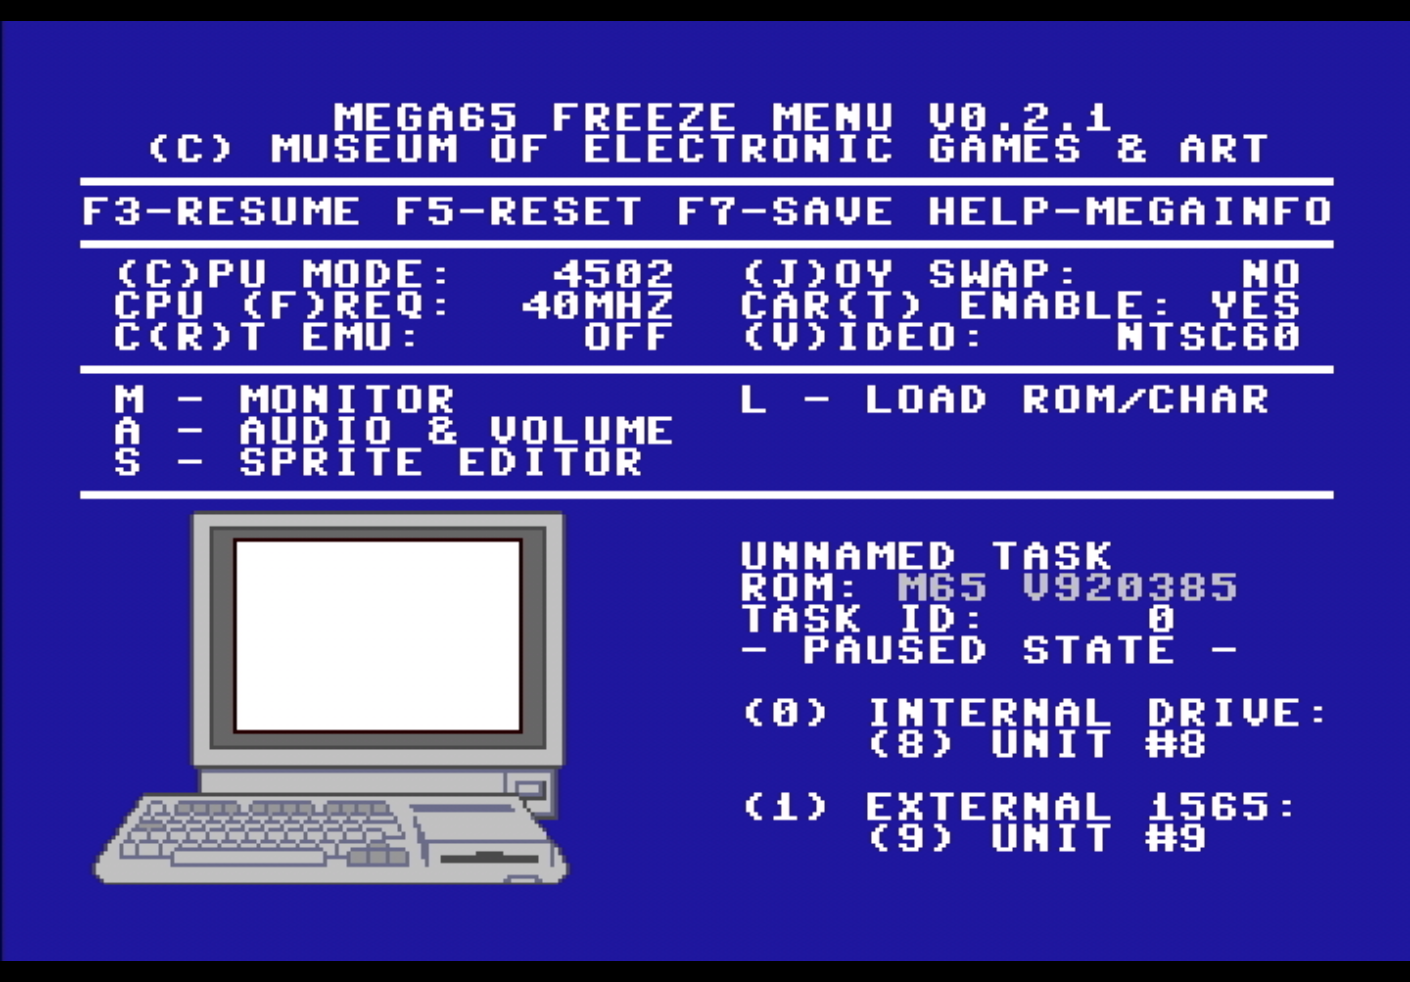
\includegraphics[width=0.7\linewidth]{images/freezer.png}
\end{center}

Een functie om te onthouden tijdens het spelen van spellen is ``(J)OY SWAP''. Deze functie laat de joystickpoorten van nummer wisselen. Hebt u een joystick in poort 2 en start u een spel dat een joystick in poort 1 verwacht, dan hoeft u de joystick niet los te koppelen en opnieuw aan te sluiten. Open in plaats daarvan het Freezer-menu, druk op \megakey{J} om de poortnummers om te wisselen en hervat vervolgens uw spel.

Het menu wordt ``Freezer'' genoemd omdat de toestand van de MEGA65 bevroren blijft terwijl u het menu gebruikt. Het Freezer-menu kan meerdere freeze-toestanden opslaan en u kunt tussen deze toestanden schakelen. Om de huidige toestand op te slaan, gaat u met de rechtercursortoets naar een ongebruikt {\it freeze-slot} en drukt u vervolgens op \megakey{F7}. Wanneer de rand ophoudt met knipperen, is de toestand opgeslagen. Om een toestand te herstellen, gaat u naar het freeze-slot en drukt u op \megakey{F3} om de werking te hervatten.

Het Freezer-menu bevat diverse ingebouwde opties en voorzieningen. Zie voor meer informatie over het MEGA65-informatiehulpprogramma (``MEGAINFO'') ``De versies van de onderdelen bepalen'' op bladzijde \pageref{sec:versions}. Zie voor meer informatie over het aankoppelen van schijven en schijfimages hoofdstuk \vref{cha:using-disks}.


\section{Commodore 64-software uitvoeren}

De MEGA65 is in staat Commodore 64-software uit te voeren. Hiervoor zijn twee mogelijkheden: de ingebouwde GO64-modus en de FPGA-core {\it C64 for MEGA65}.

\subsection{GO64-modus}
\index{Commodore 64!GO64-modus}

De oorspronkelijke Commodore 65 was ontworpen om bepaalde Commodore 64-software te kunnen uitvoeren. De MEGA65 ondersteunt deze voorziening, die bekendstaat als ``GO64-modus''.

\underline{OPMERKING}: Doordat Commodore deze voorziening op deze wijze heeft ontworpen, is niet alle C64-software compatibel met deze modus. Anders dan de vergelijkbare voorziening van de Commodore 128 gebruikt de Commodore 65 een andere CPU en het is bekend dat kleine verschillen compatibiliteitsproblemen met sommige softwaretitels veroorzaken.

Er zijn drie manieren om de MEGA65 in de GO64-modus te schakelen:

\begin{itemize}
    \item Schakel de computer uit, houd de \megasymbolkey ingedrukt en schakel hem weer in.    \item Geef bij de \screentext{READY}-prompt van de MEGA65 dit commando in: \screentext{GO64} en druk op Enter. Typ \screentext{YES} wanneer daarom wordt gevraagd.\index{BASIC 65-commando's!GO64}    \item Schakel de computer uit, sluit een Commodore 64-cartridge aan op de expansiepoort en schakel de computer vervolgens weer in.
\end{itemize}

\begin{center}
  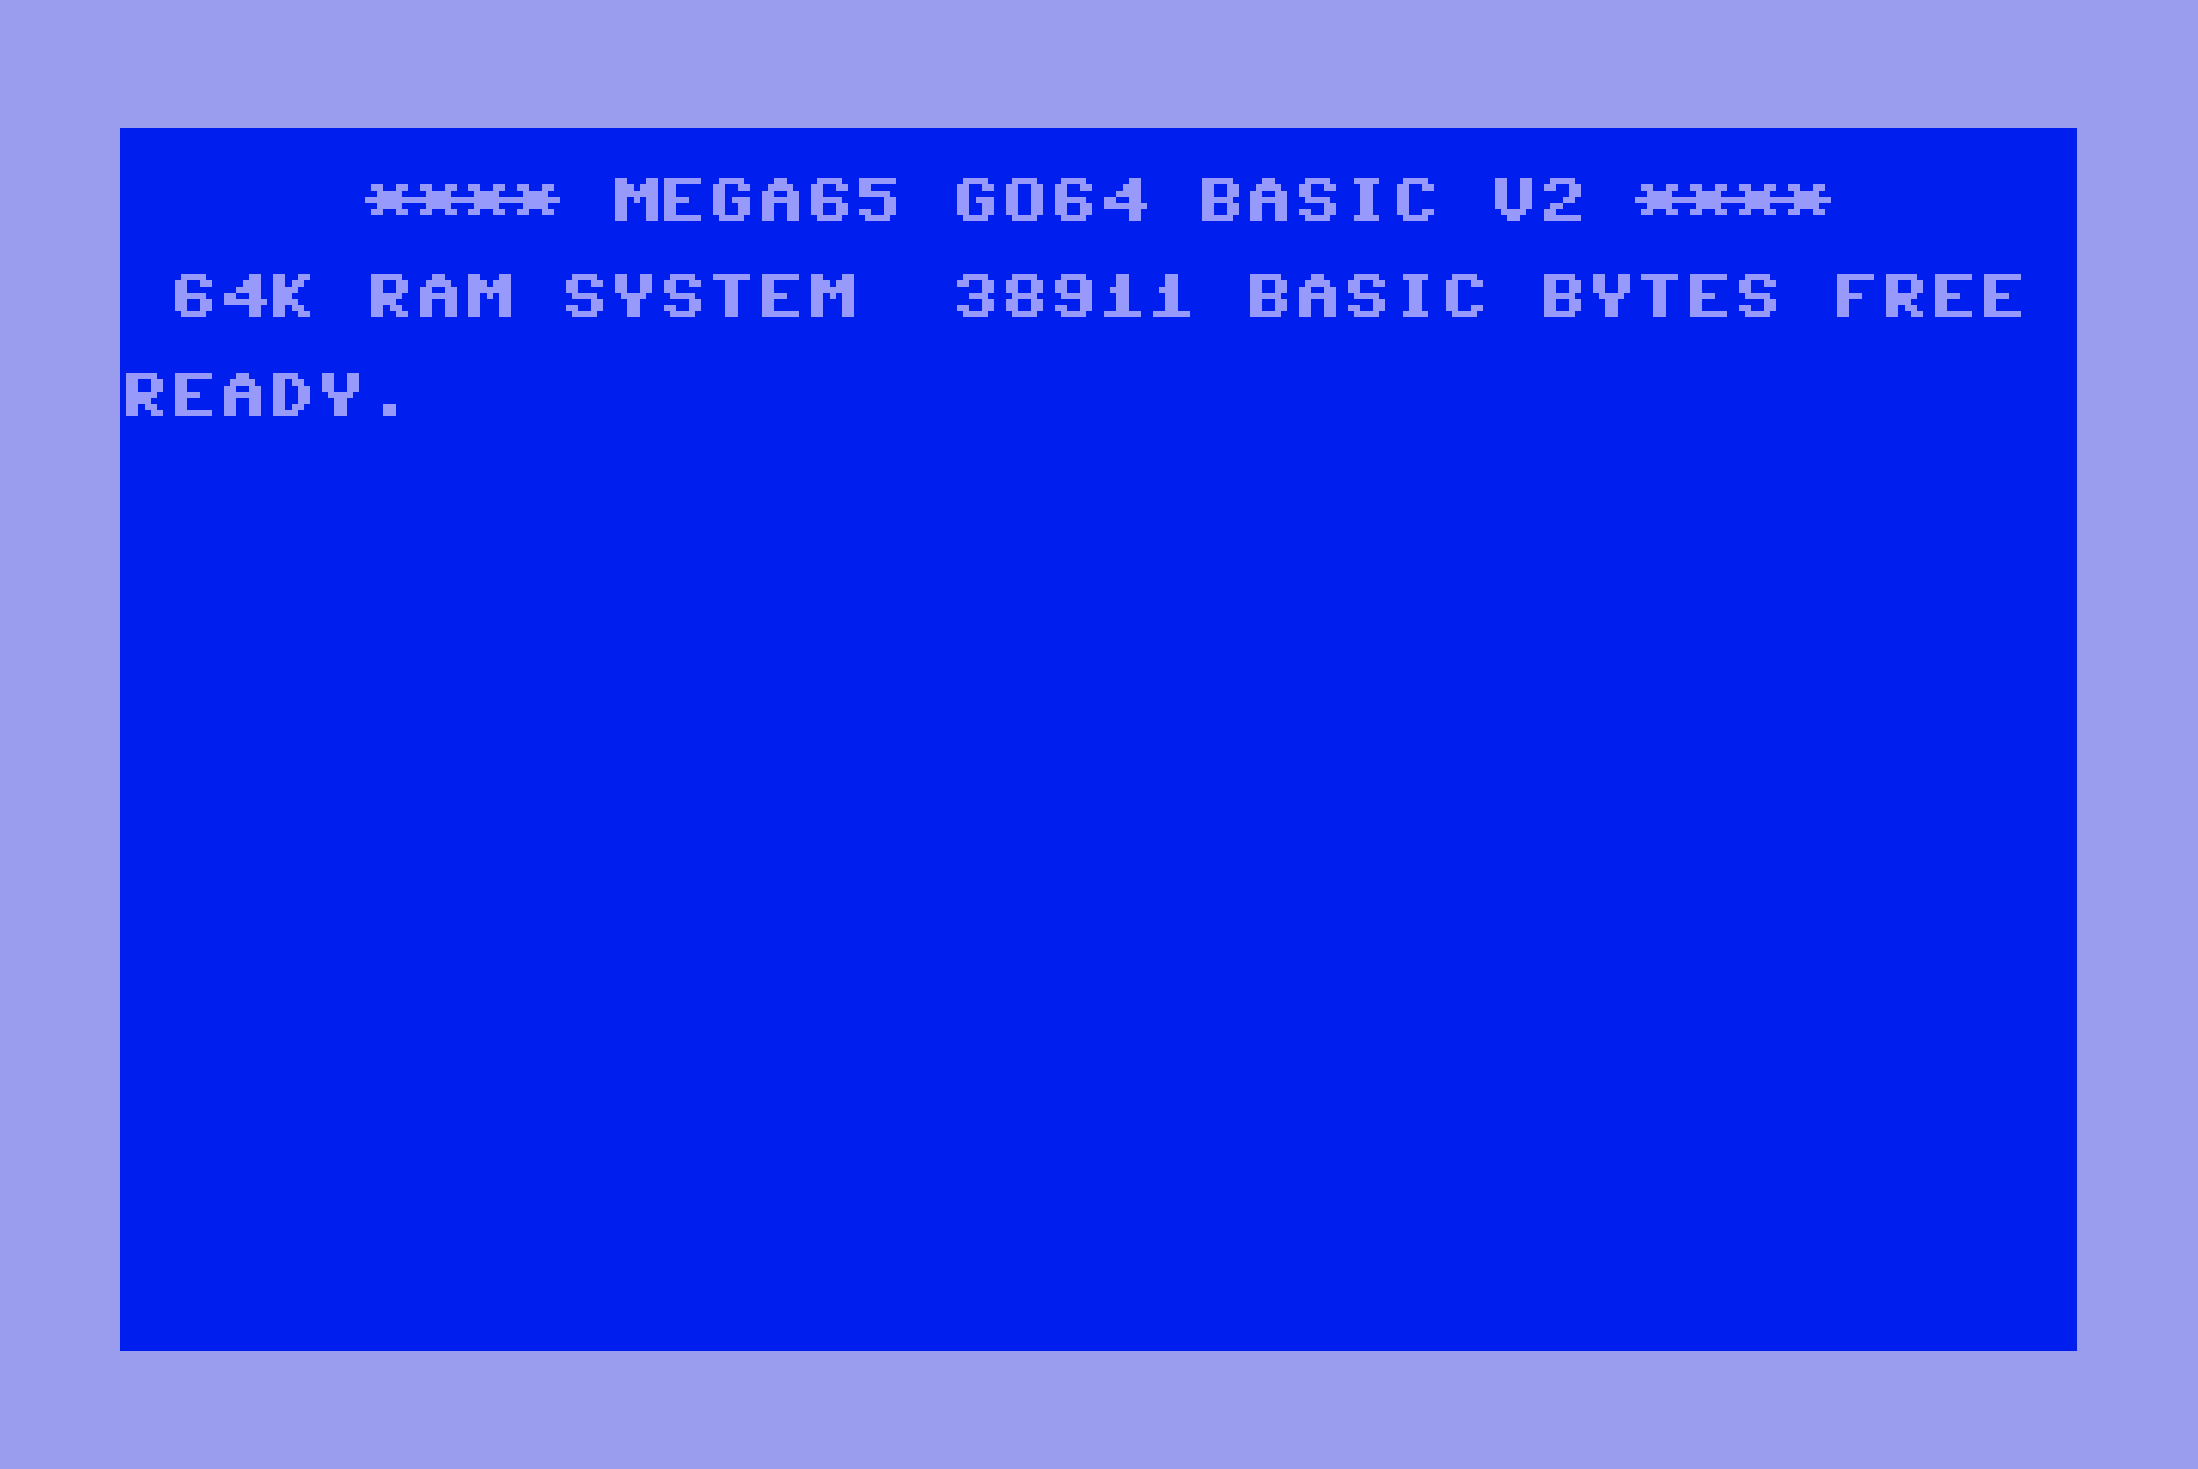
\includegraphics[width=0.7\linewidth]{images/go64.pdf}
\end{center}

De GO64-modus is eigenlijk slechts een tijdelijke herconfiguratie van de MEGA65. Alle voorzieningen van de MEGA65 blijven aanwezig, waaronder het Freezer-menu voor het aankoppelen van D81-schijfimages.

Veel Commodore 64-software is op het internet te vinden in de vorm van D64-schijfimages. De MEGA65 ondersteunt via de SD-kaart en het Freezer-menu uitsluitend D81-schijfimages. U kunt een randapparaat, zoals de SD2IEC,\index{SD2IEC device} op de IEC-poort van de MEGA65 aansluiten om D64-schijfimages te gebruiken. Zorg dat u een SD2IEC aanschaft met een onafhankelijke voeding en niet een exemplaar dat afhankelijk is van een tape-aansluiting van de Commodore 64.\footnote{Zie voor meer informatie over SD2IEC-apparaten: \url{https://www.c64-wiki.com/wiki/SD2IEC}}

\subsection{De FPGA-core ``C64 for MEGA65''}
\index{Core!C64-core}\index{Commodore 64!Core}

De FPGA-core {\it C64 for MEGA65} van MJoergen en sy2002 herschept de oorspronkelijke Commodore 64-computer op de MEGA65-hardware met een hoge mate van nauwkeurigheid. Het doet dit door de MEGA65-core volledig te vervangen door een core die de chipset van de Commodore 64 implementeert, met inbegrip van de CPU. MEGA65-voorzieningen, zoals het Freezer-menu, zijn niet beschikbaar wanneer de C64-core draait. In plaats daarvan biedt de core een eigen menu voor het aankoppelen van D64-schijfimages en andere voorzieningen. Druk op de toets \specialkey{HELP} terwijl de core draait om dit menu te openen.

% TODO: When the cartridge-to-core configuration feature is complete:
% With the C64 core installed, you can configure the MEGA65 boot process to use the core when a Commodore 64 cartridge is connected, instead of using the less-compatible GO64 mode. ...
% (Refer to chapter \vref{cha:cores})

Zie voor informatie over het installeren van FPGA-cores hoofdstuk \vref{cha:cores}. Om de core {\it C64 for MEGA65} te downloaden en de belangrijke installatie-instructies te lezen, zie: \url{https://github.com/MJoergen/C64MEGA65}
